\documentclass[pdflatex,a4paper,10pt,ja=standard]{bxjsarticle}

\usepackage[pdftex]{graphicx}
\usepackage[table]{xcolor}
\usepackage{cprotect}
\usepackage{amsmath,amssymb}
\usepackage{mathtools}
\usepackage{caption}
\usepackage{siunitx}
\usepackage{geometry}
\usepackage{color}
\usepackage{hyperref}
\usepackage{minted}
\usepackage{booktabs}
\usepackage{fancyvrb}
\usepackage{longtable}
\usepackage{comment}
\usepackage[english]{babel}
\usepackage[backend=biber,autocite=superscript,style=phys,articletitle=false,biblabel=brackets,chaptertitle=false,pageranges=false]{biblatex}
\addbibresource{ref.bib}

\geometry{left=25mm,right=25mm,top=30mm,bottom=30mm}
\def\vec#1{\mbox{\boldmath $#1$}}

%\title{拡張KAPSELドキュメント\textcolor{red}{(rev. 3.2)}}

\graphicspath{{./figures/}}
\captionsetup[figure]{labelformat={default},labelsep=period,name={Figure~}}
\captionsetup[table]{labelformat={default},labelsep=period,name={Table~}}

\SaveVerb{verb_exp}|explicit_scheme|
\SaveVerb{verb_imp}|implicit_scheme|
\SaveVerb{verb_landau}|Landau|
\SaveVerb{verb_flory_huggins}|Flory_Huggins|
\SaveVerb{verb_dc}|DC|
\SaveVerb{verb_ac}|AC|
\SaveVerb{verb_spherical_particle}|spherical_particle|
\SaveVerb{verb_chain}|chain|
\SaveVerb{verb_rigid}|rigid|
\SaveVerb{verb_npx}|NPX|
\SaveVerb{verb_npy}|NPY|
\SaveVerb{verb_npz}|NPZ|
\SaveVerb{verb_factor}|factor|
\SaveVerb{verb_gts}|GTS|
\SaveVerb{verb_num_snap}|Num_snap|
\begin{document}

% cover page ------------
\thispagestyle{empty}
{\centering
\vspace*{15truemm}
{\LARGE \textbf {フィラー充填系コンポジットシミュレータ}}\\
\vspace*{5truemm}
{\Huge \textbf {拡張KAPSEL}}\\
\vspace*{5truemm}
{\LARGE \textbf {Version 1.0u2m}}\\
\vspace*{140truemm}
{\Large \textbf {超先端材料超高速開発基盤技術プロジェクト}}\\
\vspace*{3truemm}
{\Large \textbf {Apr. 1 2019}}\\
}
\clearpage
\thispagestyle{empty}

\section*{執筆者}
尾崎弘人

\section*{拡張部プログラム開発者}
尾崎弘人,齋藤健

\section*{謝辞}
このプログラムの拡張部分は,国⽴研究開発法⼈新エネルギー・産業技術総合開発機構(NEDO)の委託業務(P16010)により開発されたものです.
\\
\\
Copyright \textcopyright 2019 AIST and ADMAT. All rights reserved.

\clearpage

\addtocounter{page}{-2}
%\maketitle
\section{拡張KAPSELの機能}
KAPSEL(\underline{K}yoto \underline{A}dvanced \underline{P}article \underline{S}imulator for \underline{EL}ectro-hydrodynamics)は,京都大学山本量一教授により開発が進められている,粒子を含む固液二相流の直接数値計算を行えるシミュレータである\autocite{kapsel,nakayama2005simulation}.
本シミュレータを用いることで,微粒子の沈降ダイナミクスやコロイド分散系のレオロジー,荷電コロイド粒子の電気泳動といった動的現象を高精度かつ高効率で計算することができる.

NEDO:超先端材料超高速開発基盤技術プロジェクトでは,上記KAPSELを基礎として,新たに二成分流体対応およびMPIによるノード間並列に対応した拡張KAPSELを開発した.
拡張KAPSELの実行モジュールと新規機能の一覧を以下に示す.各実行モジュールの入力UDFファイルは共通化されており,実行時のコマンドを変えることで,切り替えが可能となっている.
\begin{enumerate}
    \item 拡張KAPSEL(二成分流体対応/粒子間相互作用拡張): \verb|kapsel_u2m|
    \begin{itemize}
        %\item 初期流れ場なしの差分法版Navier--Stokesシミュレーション
        \item 初期流れ場なしの二成分流体シミュレーション(粘度比導入可能)
        %\item Lees--Edwards境界条件によるせん断流あり差分法版Navier--Stokesシミュレーション
        \item Lees--Edwards境界条件によるせん断流ありの二成分流体シミュレーション(粘度比導入可能)
        \item 巨視的な粒子間に働く相互作用に関する拡張
    \end{itemize}
    \item 拡張KAPSEL(MPI並列対応): \verb|kapsel_u2m_mpi|
    \begin{itemize}
        \item MPI並列計算(二成分流体対応を除く)
    \end{itemize}
\end{enumerate}

\section{インストール}
本章では,拡張KAPSELを実行するための環境設定とビルド方法について概説する.
拡張KAPSELの実行環境は,LinuxあるいはCygwinを導入したWindowsを想定している.
ここに示すディレクトリ名やファイルバージョンは,各自の実行環境に合わせて適宜読み替えていただきたい.

\subsection{OCTAのインストール・libplatformのビルド}
拡張KAPSELでは,入出力ファイルにUDFファイルを使用することから,OCTAに含まれるlibplatformが必要となる.
OCTAのインストール後,libplatformのビルドを行う.
Linuxでは,
\begin{minted}{console}
    $ cd /usr/local/OCTA8/GOURMET/src
    $ make clean
    $ ./configure
    $ make
    $ make install
\end{minted}
WindowsのCygwin\autocite{cygwin}環境では,
\begin{minted}{console}
    $ ln -s /cygdrive/c/OCTA8 /usr/local/OCTA8
    $ cd /usr/local/OCTA8/GOURMET/src
    $ make clean
    $ ./configure
    $ make
    $ make install
\end{minted}
\begin{comment}
Macでは,
\begin{minted}{console}
    $ cd /usr/local/OCTA8/GOURMET/src
    $ make distclean; make clean
    $ ./configure CC=gcc-7 CXX=g++-7
    $ make
    $ sudo make install
    $ mv ../lib/macosx/libplatform.a ../lib/macosx/libplatform_gcc-7.a
\end{minted}
\end{comment}
でビルドが可能である.
\begin{comment}
また,コンパイラとしてgccではなくclangを使用したい場合,以下のオプションを与える.
\begin{minted}{console}
    $ ./configure CC=clang CXX=clang++
\end{minted}
\end{comment}
KAPSELの利用に伴うlibplatformのビルドの詳細は,KAPSEL公式ホームページ内のSTEP 2: Build ``libplatform''の項目\autocite{kapsel_install}を参照いただきたい.

\subsection{HDF5のインストール}
HDF5(Hierarchical Data Format 5)は,大容量のデータを階層的に扱うファイル形式である\autocite{hdf5}.
オリジナルのKAPSELではオプションとしてHDF5出力を選択できたが,二成分流体対応の拡張KAPSELでは大容量のフィールドデータを扱う都合上,実行モジュールのコンパイル時において,HDF5の導入を必須としている.
\begin{comment}
HDF5は公式ホームページでソースコードが提供されており\autocite{hdf5_sourcecode},これを展開後ビルドすることで導入できる.
\begin{minted}{console}
    $ cd hdf5-($VERSION) 
    $ ./configure --prefix=/usr/local
    $ make
    $ make check
    $ make install
\end{minted}
ここで,\verb|($VERSION)|はバージョンを表す.
また,Linuxであれば,パッケージ管理システムによって導入することもできる.
\end{comment}
Linuxであれば,パッケージシステムによって導入することができる.
以下は,CentOSでのインストール例である.
\begin{minted}{console}
    $ sudo yum -y install hdf5-devel
\end{minted}
WindowsのCygwin環境では,公式ホームページ\autocite{cygwin}から入手できるGUIインストーラを利用することで,関連するパッケージ\verb|libhdf5-devel|と\verb|libhdf5cpp-11|を導入できる(図\ref{fig:cygwin_install}).
\begin{figure}[htbp]
    \centering
    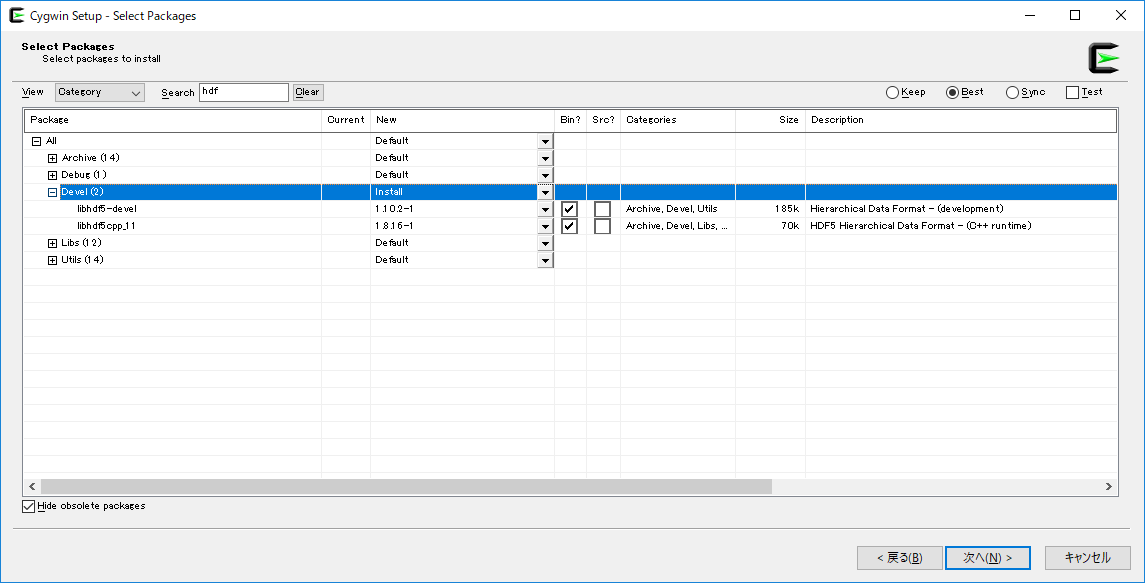
\includegraphics[width=14truecm]{cygwin_ss.png}
    \caption{Cygwinインストーラを利用したHDF5の導入}
    \label{fig:cygwin_install}
\end{figure}

\subsection{FFTWのインストール(オプション)}
\label{sec:fftw}

FFTW\autocite{fftw}は,高速なFFT計算を可能とする計算ライブラリである.
オリジナルのKAPSELでは,ver.3.40からFFTWライブラリを利用した計算に対応している.
二成分流体対応の拡張KAPSELでも同様に利用可能である.

FFTWの導入方法は以下の通りである.
Linuxの場合,公式ホームページ\autocite{fftw_download}よりソースコードをダウンロード後,以下のコマンドで導入できる.
\begin{minted}[breaklines]{console}
    $ ./configure CFLAGS="-O3" FFLAGS="-O3" --enable-openmp --enable-threads --enable-shared --disable-fortran
    $ make
    $ make install
\end{minted}
また,コンパイラとしてiccを利用したい場合,
\begin{minted}[breaklines]{console}
    $ ./configure CC=icc CXX=icpc CFLAGS="-O3" FFLAGS="-O3" --enable-openmp --enable-threads --enable-shared --disable-fortran --enable-sse2 --enable-avx --enable-avx2
    $ make
    $ make install
\end{minted}
である.
WindowsのCygwin環境では,Cygwinインストーラより\verb|libfftw3-devel|パッケージをインストールすることで導入できる.

\begin{comment}
Macの場合,ソースコード\autocite{fftw_download}をダウンロード後,以下のコマンドで導入できる.
\begin{minted}[breaklines]{console}
    $ ./configure CC=gcc-7 CXX=g++-7 CFLAGS="-O3" FFLAGS="-O3" --enable-openmp --enable-threads --enable-shared --disable-fortran
    $ make
    $ sudo make install
\end{minted}
\end{comment}

\subsection{Lisライブラリのインストール(オプション)}
\label{sec:lis}

二成分流体対応/粒子間相互作用拡張の拡張KAPSELでは,陰解法ソルバーが実装されている(詳細は\ref{sec:theory}章に示す).
その陰解法の反復解法において,並列反復解法ライブラリLisを利用した計算が可能である\autocite{lis}.
Lisには数多くの反復解法と前処理法が実装されており,これを利用することで,シミュレーション条件に応じて適切な解法を選択できるようになる.
尚,Lisライブラリの導入はコンパイル時において必須ではなく,導入していない場合でも拡張KAPSELの全ての機能を利用できる.
Lisの導入方法を以下に示す.
Lisには多数の導入オプションがあるが,その詳細は公式ユーザーガイド\autocite{lis_document}を参照いただきたい.

Linuxの場合,まずダウンロードしたソースコードを展開する.
\begin{minted}{console}
    $ unzip lis-($VERSION).zip
\end{minted}
ここで,\verb|($VERSION)|はバージョンを表す.
作成されたサブディレクトリ内に移動し,実行モジュールを生成する.
\begin{minted}{console}
    $ cd lis-($VERSION)
    $ ./configure
    $ make
    $ make install
\end{minted}

Windowsの場合,ダウンロードしたソースコードを展開後,\verb|lis-($VERSION)\win|に移動し,
\begin{minted}{console}
    > configure.bat
\end{minted}
を実行する.
実行ファイルは,同じディレクトリにおいて,
\begin{minted}{console}
    > nmake
\end{minted}
を実行することで,作成される.
\begin{minted}{console}
    > nmake install
\end{minted}
とすることで,各種ファイルがそれぞれ\verb|($INSTALLDIR)\lib|,\verb|($INSTALLDIR)\bin|,\verb|($INSTALLDIR)\include|,\verb|($INSTALLDIR)\doc|に導入される.

\subsection{拡張KAPSELのインストール}

二成分流体対応/粒子間相互作用拡張KAPSELのソースコードは\verb|kapsel_u2m.zip|に,MPI並列対応KAPSEL\verb|kapsel_u2m_mpi.zip|にまとめられている.
いずれにおいてもインストールの作業はほぼ同様である.
以下では,二成分流体対応/粒子間相互作用拡張KAPSEL(\verb|kapsel_u2m|)を例に説明する.

まず,ダウンロードしたソースコードを展開する.

\begin{minted}{console}
    $ unzip kapsel_u2m.zip
\end{minted}

次に,展開してできるディレクトリに移動し,KAPSELの実行モジュールをビルドする.
\begin{minted}{console}
    $ cd kapsel_u2m
    $ make
\end{minted}

ビルドするにあたり,makefileにおいてPATHの設定を行うとともに,環境に合わせていくつかのオプションを選択する必要がある.
\verb|ENV|オプションでは,使用するコンパイラが設定できる.
\verb|FFT|オプションでは,使用するFFTライブラリが選択できる.
\verb|HDF5|オプションは二成分流体対応の拡張KAPSELでは\verb|ON|でなければならない.
二成分流体対応の拡張KAPSELでは,\verb|LIS|オプションを\verb|ON|にすると,陰解法ソルバーにおいてLisが使用される.
Lisの設定については,\ref{sec:lis_settings}節に示す.
設定できる\verb|ENV|及び\verb|FFT|オプションの一覧を以下に示す.

\begin{enumerate}
    \item 二成分流体対応/粒子間相互作用拡張KAPSEL(\verb|kapsel_u2m|)
    \begin{enumerate}
        \item Linux ENV
        \begin{itemize}
        \item \verb|ENV = GCC| (GCC コンパイラ)
        \item \verb|ENV = ICC| (Intel C++ Compiler)
        \item \verb|ENV = ICC_OMP| (Intel C++ Compiler + OpenMP)
        \end{itemize}
        \item Windows ENV
        \begin{itemize}
        \item \verb|ENV = CYGWIN| (Cygwin)
        \item \verb|ENV = CYGWIN_OMP| (Cygwin + OpenMP)
        %\item \verb|ENV = MINGW64| (MinGW 64bit)
        %\item \verb|ENV = MINGW| (MinGW)
        \end{itemize}
        %\item MAC ENV
        %\begin{itemize}
        %\item \verb|ENV = GCC_MAC| (GCC コンパイラ)
        %\item \verb|ENV = CLANG| (Clang コンパイラ)
        %\end{itemize}
        \item FFT (各OS共通オプション)
        \begin{itemize}
            \item \verb|FFT = FFTW| (FFTW)
            \item \verb|FFT = IMKL| (Intel Math Kernel Library)
            \item \verb|FFT = OOURA| (大浦版FFT\autocite{ooura_fft})
        \end{itemize}
    \end{enumerate}

    \item MPI並列対応KAPSEL(\verb|kapsel_u2m_mpi|)
    \begin{enumerate}
        \item Linux
        \begin{itemize}
            \item \verb|ENV = ICC_MKL_MPI| (Intel C++ Compiler + Intel MPI)
        \end{itemize}
    \end{enumerate}
\end{enumerate}
FFTWを利用するためには,\ref{sec:fftw}節に記したFFTWのインストールが必要となる.
また,Intel C++ CompilerとIntel Math Kernel Library(IMKL)が導入されている環境に限り,\verb|ENV = ICC|と\verb|FFT = IMKL|の設定を利用できる.
FFTWとIMKLのいずれも導入していない場合,KAPSELに組み込まれている大浦版FFT\autocite{ooura_fft}を利用するとよい.
%
%上記の手順により,KAPSELの実行モジュールが生成されていることを確認する.

\section{拡張KAPSELの実行とシミュレーション結果の確認}
\label{sec:kapsel_sample}
前節で生成されたKAPSELの実行モジュールの動作確認を行うため,サンプルのUDFファイルを使った短時間のシミュレーションを行う.

\subsection{二成分流体対応/粒子間相互作用拡張KAPSELの実行}

\verb|kapsel_u2m.zip|を展開して出来るディレクトリに,\verb|sample|ディレクトリが存在する.
以下のコマンドにより,そのディレクトリに移動し,拡張KAPSELの動作確認を行う.
\begin{minted}{console}
    $ cd sample
    $ ../kapsel_u2m -Iinput.udf -Ooutput.udf -Ddefine.udf -Rrestart.udf
\end{minted}
シミュレーションが正しく終了すると,以下のような出力が表示される.
計算時間は実行環境によって異なるが,本サンプルの場合数十秒程度で終了するはずである.
\begin{minted}{text}
    #Simulation has ended!
    #Total Running Time (s):      11.89
    #                   (m):       0.20
    #                   (h):       0.00
    #Average Step Time  (s):       0.01
    #                   (m):       0.00
    #                   (h):       0.00
\end{minted}
また,シミュレーションの終了とともに,いくつかのファイルが新たに生成される.
\verb|output.udf|ファイルには,シミュレーションで得られた各ステップにおける粒子運動と相分離オーダーパラメータが出力されている.
このファイルをGOURMETで開くことで,シミュレーション結果を確認できる.
\verb|sample|ディレクトリには,GOURMETで粒子と相分離構造を可視化するためのPythonスクリプトである\verb|gourmet_particle_field_show.py|が用意されている.
GOURMETを起動し,\verb|output.udf|ファイルを読み込んだ後,下部のPythonパネルに\verb|gourmet_particle_field_show.py|を読み込む.
これを実行すると,新たな描画ウィンドウが開き,シミュレーション結果をアニメーションとして確認することができる(図\ref{fig:gourmet_output}).
図では,粒子が白の球として,また流体界面が青い等値面として表されている.

\begin{figure}[htbp]
    \centering
    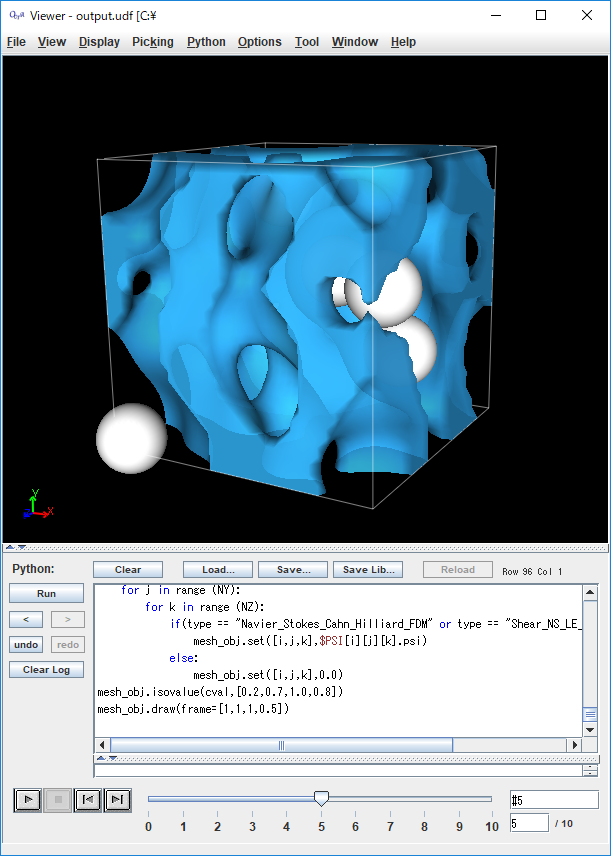
\includegraphics[width=8truecm]{gourmet_output_ss.png}
    \caption{GOURMETによるシミュレーション結果の可視化}
    \label{fig:gourmet_output}
\end{figure}

\verb|.h5|の拡張子のファイルには,各出力ステップにおけるシミュレーションデータがHDF5バイナリ形式で保存されている.
保存されたシミュレーションデータは,h5dumpコマンドを使うことで,端末上で直接確認できる.
\begin{minted}{console}
    $ h5dump orderparam_0.h5
\end{minted}
\verb|.xmf|の拡張子のファイルは,XDMF(eXtensible Data Model and Format)ファイルである.このファイルには,上記のHDF5ファイルに保存されたデータの計算点の空間配置等の幾何構造が保存されており,HDF5ファイルのデータと共に解析に使用される.
このファイルは,ParaView\autocite{paraview}等の可視化ソフトで開くことができる.
本ディレクトリには,ParaViewで解析する場合のサンプルファイル(state file)を用意している.
ParaViewで\verb|pv_sample.pvsm|を開き,以下の手順に従い\verb|sample|ディレクトリのパスを指定することで,シミュレーション結果が可視化できる.
ParaViewでpvsmファイルを開くと,\verb|Load State Options|の設定画面が現れる.
その中で\verb|Load State Data File Options|の項目を\verb|Search files under specified directory|に設定し,
\verb|Data Directory|に\verb|sample|ディレクトリの絶対パスを指定する.
図\ref{fig:paraview}にParaViewによるシミュレーションの可視化の結果を示す.

\begin{figure}[htbp]
    \centering
    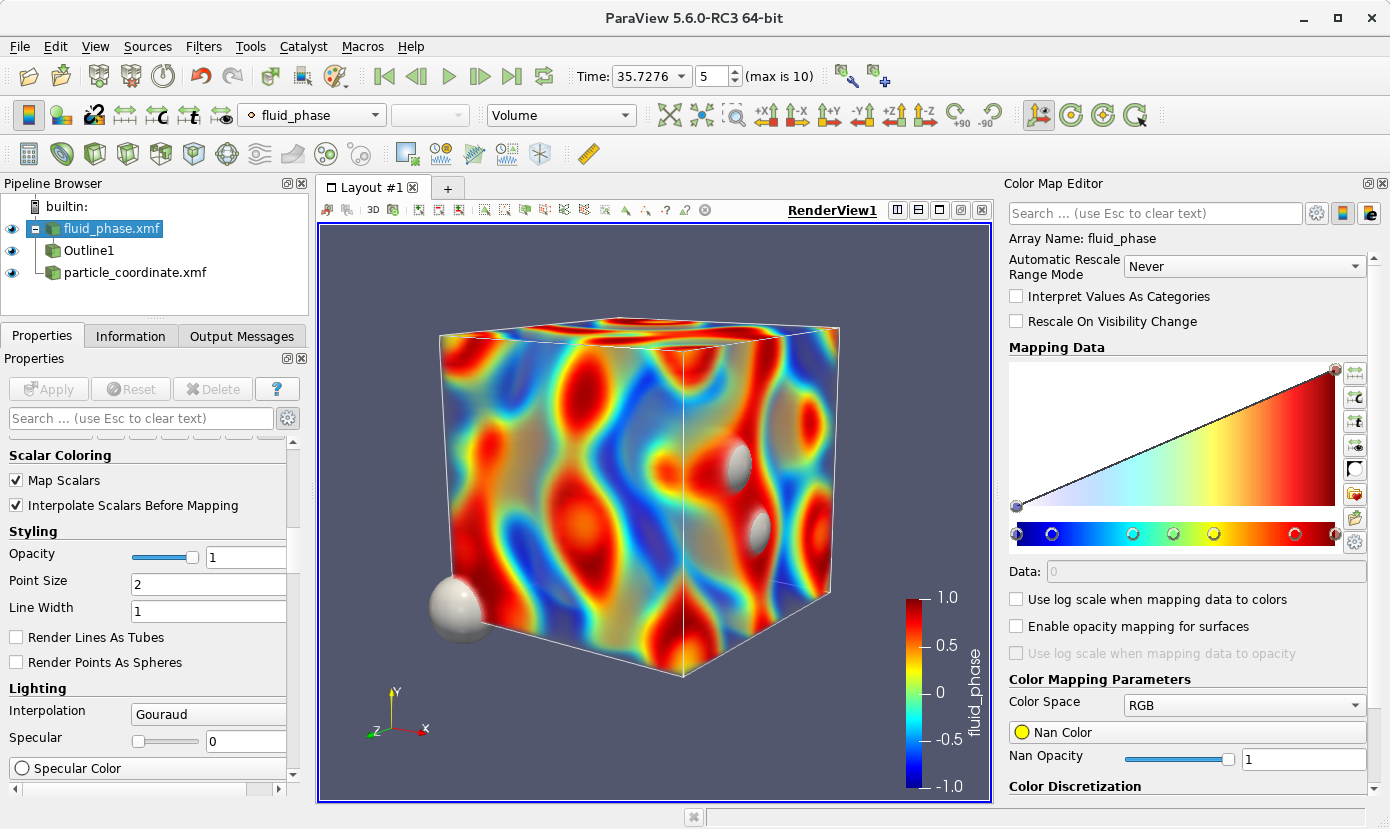
\includegraphics[width=13truecm]{paraview_ss.png}
    \caption{Paraviewによるシミュレーション結果の可視化}
    \label{fig:paraview}
\end{figure}

また,得られた結果をPythonスクリプトで読み込み,別途解析することもできる.
本ディレクトリには,相分離構造の静的構造因子$S(q)$を計算するPythonスクリプトが同梱されている.
Pythonパッケージのh5py,scipy,matplotlibが導入された環境で以下のコマンドを実行することで,各時間ステップにおける$S(q)$のグラフが逐次得られる(図\ref{fig:sq_vs_q}).

\begin{minted}{console}
    $ python sq_analysis.py
\end{minted}

\begin{figure}[htbp]
    \centering
    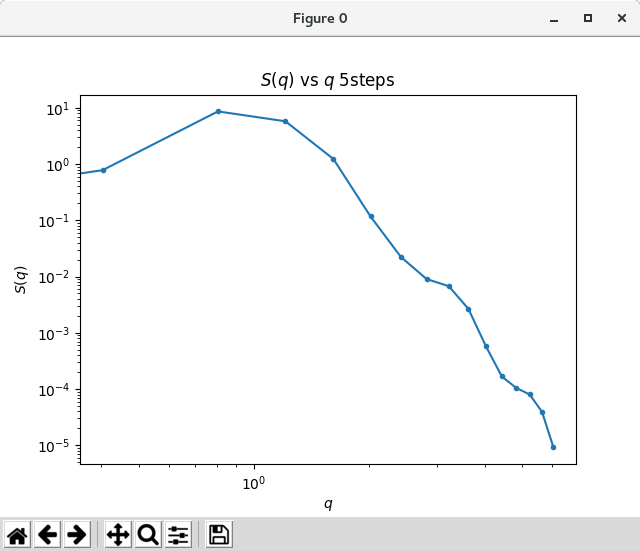
\includegraphics[width=9truecm]{sq_vs_q.png}
    \caption{Pythonスクリプトによる解析例: 静的構造因子$S(q)$を波数$q$に対してプロットしている($5$ステップ目の結果を示す).}
    \label{fig:sq_vs_q}
\end{figure}

その他いくつか解析用のPythonスクリプトが\verb|python|ディレクトリに同梱されている.
各解析スクリプトの使用方法は,同ディレクトリ内のドキュメントを参照頂きたい.

\subsection{MPI並列対応の拡張KAPSELの実行}

\verb|kapsel_u2m_mpi.zip|を展開して出来るディレクトリに,\verb|sample|ディレクトリが存在する.
以下のコマンドにより,そのディレクトリに移動し,拡張KAPSELのサンプル動作確認を行う.
%これは,オリジナルのKAPSELのサンプルファイルと同じものである.
\begin{minted}[breaklines]{console}
    $ cd sample
    $ mpirun -n 4 ../kapsel_u2m_mpi -X2 -Y2 -Iinput.udf -Ooutput.udf -Ddefine.udf -Rrestart.udf
\end{minted}

MPI並列対応の拡張KAPSELの実行時には,オリジナルのKAPSELの引数に加えて,新たに\verb|-X|と\verb|-Y|のオプションを設定する必要がある.
これは,それぞれ$x$及び$y$方向の空間領域分割数を表し,それらのオプションで指定された数字の積が
\verb|-n|で指定されるMPI並列数と等しい必要がある.
上記の例では,$x$及び$y$方向においてそれぞれ$2$分割された$4$並列のシミュレーションが実行される.
プログラムの制約上,\verb|-X|と\verb|-Y|で与える空間領域分割数は$2^{n} ~ (n = 0, 1, 2, ...)$の値のみ対応しており,それ以外の値を与えた場合エラーメッセージが表示され,プログラムは終了される.
ここで実行したサンプルシミュレーションは,オリジナルのKAPSELに付属のものと同じものであり,MPI並列対応の拡張KAPSELで得られる結果はオリジナルのKAPSELの結果と同一である.

\section{理論}
\label{sec:theory}
本章では,KAPSELにおける粒子を含む流体の計算手法と拡張KAPSELにおける二成分流体の取扱いについて概説する.

\subsection{Smoothed Profile Method}
\label{sec:spm}
一般に,流体と構造体の連成解析では,移動する界面の取り扱いが問題となり,これまで数多くの手法が提案されてきた\autocite{kobayashi2003cfd,jsces2017fem}.
それらは次の2つの手法に大別できる.
1つは,移動格子を用いることで界面位置を計算領域境界として直接的に表現する手法である.
また,もう1つは,物理量とは異なる識別関数を導入し,固定計算格子上で界面を間接的に表現する手法である.
KAPSELが採用するSmoothed Profile Method(SPM)\autocite{nakayama2005simulation,iwashita2008numerical,iwashita2009short,kobayashi2011implementation,molina2016rheological}は,後者に属する手法である.
SPMでは,流体部分と粒子部分を識別する補助関数(粒子界面関数)を導入することにより,流体解析の計算格子を固定したまま,流体中の粒子運動を高効率に計算できる.
\begin{figure}[htbp]
    \centering
    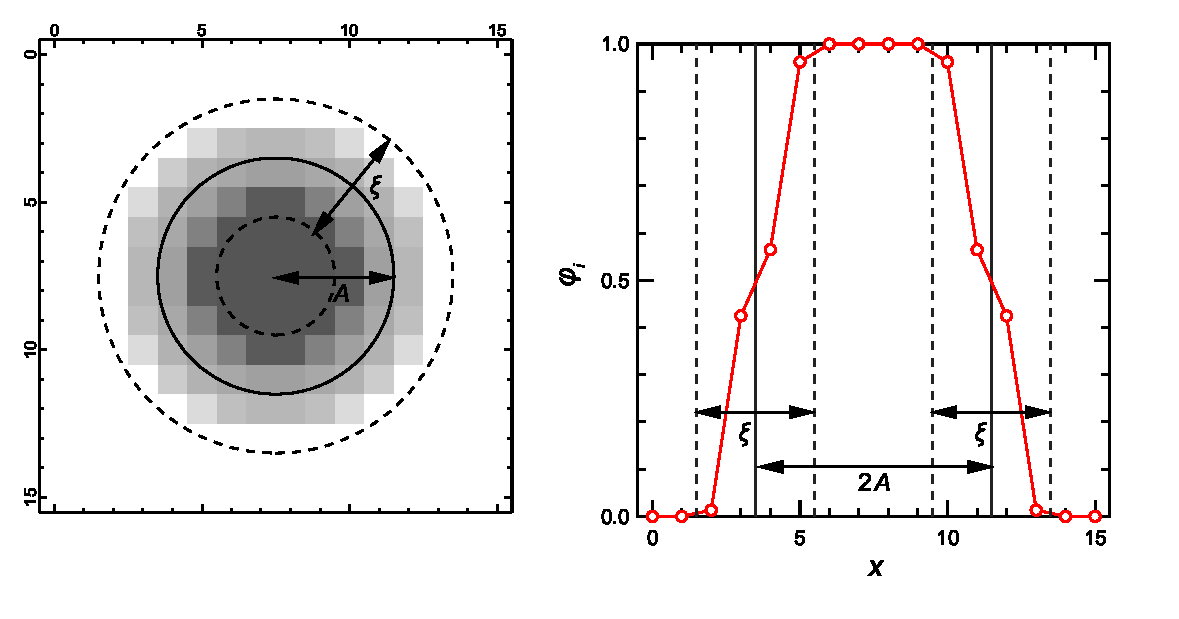
\includegraphics[width=12truecm]{phi.pdf}
    \caption{粒子界面関数の一例.
    左図は二次元での粒子界面関数を表し,$\phi_{i} =1$の粒子領域が濃い灰色で,$\phi_{i} =0$の流体領域が白色で示されている.
    右図は,粒子の中心を通る線上での粒子界面関数を表す.
    流体--粒子界面には,$0$と$1$の間の値をとる厚み$\xi$の領域が存在する.}
    \label{fig:phi}
\end{figure}
図\ref{fig:phi}は,$i$番目の粒子の界面関数$\phi_{i}$の一例である.
ここで,粒子半径は$A$としている.
左図は2次元における粒子界面関数を表しており,右図は粒子中心を通る線上での界面関数を表している.
この界面関数は,流体領域で$\phi_{i} = 0$,粒子領域で$\phi_{i} = 1$をとる関数であり,その間は厚み$\xi$の界面領域をもつ滑らかに変化する連続関数である.
粒子界面関数は様々な定式化が提案されている\autocite{nakayama2005simulation}が,KAPSELのデフォルトの設定では,
\begin{align}
    \phi_{i}(\vec{x}) &= g(|\vec{x} - \vec{R}_{i}|) \\
    g(x) &=  \frac{h[(A+\xi/2)-x]}{h[(A+\xi/2)-x] + h[x - (A -\xi/2)]} \\
    h(x) &= \begin{cases}
    \exp(-\Delta^2/x^2) & x \geq 0 \\
    0 & x < 0
    \end{cases}
\end{align}
となっている.
ここで,$\vec{x}$は空間座標,$\vec{R}_{i}$は$i$番目の粒子位置座標である.
また,$\Delta$ は格子幅を表す.
KAPSELでは,3次元全ての方向において格子幅は一定としている.
系に粒子が$N$個存在するとき,系全体の粒子界面関数$\phi$は,
\begin{align}
    \phi = \sum_{i}^{N} \phi_{i}
\end{align}
で与えられる.
この粒子界面関数により計算領域中のどの部分に粒子が存在するかを識別できる.
また,SPMでは計算領域の速度場$\vec{u}$を,$\phi$を使って,
\begin{align}
    \vec{u} &= \phi \vec{u}_{\mathrm p} + (1-\phi) \vec{u}_{\mathrm f} 
\end{align}
と定義する.
ここで,$\vec{u}_{\mathrm p}$と$\vec{u}_{\mathrm f}$は,それぞれ粒子部分の速度場と流体部分の速度場を表す.
粒子部分の速度場$\vec{u}_{\mathrm p}$は,各粒子の並進速度$\vec{V}_{i}$と角速度$\vec{\Omega}_{i}$と対応するように,以下のように決められる:
\begin{align}
    \phi(\vec{x},t) \vec{u}_{\mathrm p}(\vec{x},t) = \sum_{i=1}^{N}\left\{\vec{V}_{i}(t) + \vec{\Omega}_{i}(t) \times [\vec{x} - \vec{R}_{i}(t)] \right\} \phi_{i}(\vec{x},t) 
    \label{eq:phi_particle}
\end{align}
このようにして得られた速度場$\vec{u}$は,界面で滑りなしかつ流体の浸透もないとすれば,連続の式
\begin{align}
    \vec{\nabla} \cdot \vec{u} = 0
\end{align}
を満たす.
SPMでは速度場$\vec{u}$がNavier--Stokes(NS)方程式に従うとする:
\begin{align}
    \frac{\partial \vec{u}}{\partial t} + (\vec{u} \cdot \vec{\nabla}) \vec{u} & = - \frac{1}{\rho} \vec{\nabla} p + \nu \nabla ^2 \vec{u} + \phi \vec{f}_{\mathrm p}
    \label{eq:navier_stokes}
\end{align}
ここで,$\rho$は流体の密度,$p$は圧力である.
$\nu$は動粘性係数であり,ここでは場所によらない定数として扱う.
また,$\phi \vec{f}_{\mathrm p}$は,粒子が流体に及ぼす体積力項であり,粒子部分の速度場が式(\ref{eq:phi_particle})と一致するように流体に印加される.
これは粒子の剛直性を保証する力である.

一方,$i$番目の粒子の並進速度$\vec{V}_{i}$と角速度$\vec{\Omega}_{i}$に関する運動方程式は,
\begin{align}
    M_{\mathrm p}  \frac{d \vec{V}_{i}}{d t} &= \vec{F}_{i}^{\mathrm H} + \vec{F}_{i}^{\mathrm {other}} + \vec{G}_{i}^{\mathrm V} \label{eq:translational_motion}\\
    I_{\mathrm p} \cdot \frac{d \vec{\Omega}_{i}}{d t} &= \vec{N}_{i}^{\mathrm H} + \vec{N}_{i}^{\mathrm {other}} + \vec{G}_{i}^{\mathrm \Omega} \label{eq:rotational_motion}
\end{align}
で与えられる.
ここで,$M_{\mathrm p}$は粒子の質量,$I_{\mathrm p}$は慣性モーメント,$\vec{F}_{i}^{\mathrm H}$と$\vec{N}_{i}^{\mathrm H}$は粒子が流体から受ける力とトルク,$\vec{F}_{i}^{\mathrm {other}}$と$\vec{N}_{i}^{\mathrm {other}}$は流体以外からの力とトルクをそれぞれ表す.
粒子が流体から受ける力を計算するため,応力テンソルの表面積分を行う必要があるが,SPMではこれを粒子内部の仮想流体領域に印加される体積力の体積積分に置き換えて計算する:
\begin{align}
    \vec{F}_{i}^{\mathrm{H}} &= - \int_{V_{\mathrm p}} \rho \phi_{i} \vec{f}_{\mathrm p} d \vec{x} \\
    \vec{N}_{i}^{\mathrm{H}} &= - \int_{V_{\mathrm p}} \rho (\vec{x} - \vec{R}_{i}) \times \phi_{i} \vec{f}_{\mathrm p} d \vec{x}
\end{align}
ここで,$V_{\mathrm p}$は粒子体積を表している.
これにより,SPMでは粒子--流体間の運動量交換が漏れなく行われる.
また,式(\ref{eq:translational_motion})(\ref{eq:rotational_motion})中の$\vec{G}_{i}^{\mathrm V}$と$\vec{G}_{i}^{\mathrm \Omega}$は,熱揺らぎによって粒子に働くランダム力とトルクを表し,白色雑音としてそれぞれ与えられる:
\begin{align}
    \begin{cases}
    \langle \vec{G}_{i}^{\mathrm V} (t) \rangle = \vec{0} \\
    \langle \vec{G}_{i}^{\mathrm V} (t) \cdot \vec{G}_{j}^{\mathrm V} (0)\rangle = 3 k_{\mathrm B} T \alpha^{\mathrm V} \delta(t) \delta_{ij} 
    \end{cases}\\
    \begin{cases}
        \langle \vec{G}_{i}^{\mathrm \Omega} (t) \rangle = \vec{0} \\
        \langle \vec{G}_{i}^{\mathrm \Omega} (t) \cdot \vec{G}_{j}^{\mathrm \Omega} (0)\rangle = 3 k_{\mathrm B} T \alpha^{\mathrm \Omega} \delta(t) \delta_{ij} 
        \end{cases}
\end{align}
ここで,$\langle \cdots \rangle$は統計平均を表す.
$k_{\mathrm B}$はBoltzmann定数であり,$T$は温度である.
$\delta(t)$はデルタ関数であり,$\delta_{ij}$はKroneckerのデルタである.
$\alpha^{\mathrm V}$と$\alpha^{\mathrm \Omega}$は,粒子温度を精度よく$T$とするための補正パラメータであり,通常は$\alpha^{\mathrm V} = \alpha^{\mathrm \Omega} = 1$としてよい.
精密な温度決定の詳細は,文献\autocite{iwashita2008numerical,iwashita2009short}に記されている.

SPMでは,上記の流体と粒子に関する方程式(\ref{eq:navier_stokes})--(\ref{eq:rotational_motion})を,粒子--流体間の運動量交換を考慮しながら逐次的に解き,粒子を含む固液二相流の直接数値計算を行う.

\subsection{二成分流体の取り扱い}
\label{sec:phase_separation}
\ref{sec:spm}節では,一成分の流体中の粒子を記述するSPMについて概説した.
本節では,二成分流体を扱うSPMについて説明する.
一成分流体中の粒子を扱う場合は,粒子--流体間の界面のみを考慮すればよかったが,二成分流体では新たに流体--流体間界面を表現する必要がある.
流体--流体間界面も粒子--流体間界面と同様の手法で取り扱うことができる.
つまり,新たに二成分流体を区別する識別関数$\psi$を導入し,その時間発展を記述する.
ここでは,その識別関数$\psi$を流体界面関数と呼ぶことにする.
二成分流体のダイナミクスを記述するモデルとしては,いわゆるmodel Hが知られている\autocite{hohenberg1977theory}.
拡張KAPSELでは,model HとSPMを組み合わせることで,固体粒子を含む二成分流体を扱う.

二成分流体を扱う場合,NS方程式には化学ポテンシャル勾配項が導入され,
\begin{align}
    \frac{\partial \vec{u}}{\partial t} + (\vec{u}\cdot \vec{\nabla}) \vec{u} & = - \frac{1}{\rho} \vec{\nabla} p + \frac{1}{\rho} \vec{\nabla} \cdot \eta (\vec{\nabla}\vec{u} + \vec{\nabla}\vec{u}^{\mathrm T}) - \frac{\psi}{\rho} \vec{\nabla} \mu + \phi \vec{f}_{\mathrm p}
    \label{eq:navier_stokes_model_h}
\end{align}
となる.
ここで,$\eta$は粘度であり,ここでは場所に依存する物理量として扱う.
また,上付きの${}^\mathrm{T}$は,転置行列を表す.
$\mu$は局所的に定義される化学ポテンシャルであり,Ginzburg--Landau(GL)自由エネルギー$F$の汎関数微分により与えられる: $\mu = \delta F/\delta \psi$.

また,$\psi$の時間発展は,対流項を考慮したCahn--Hilliard(CH)方程式によって記述される:
\begin{align}
    \frac{\partial \psi}{\partial t} + (\vec{u}\cdot \vec{\nabla}) \psi & = \kappa \nabla ^2 \mu
    \label{eq:cahn_hilliard}
\end{align}
ここで,$\kappa$は易動度である.

次に,自由エネルギーについて説明する.
GL自由エネルギーは,オーダパラメータ(ここでは$\psi$)に依存する関数$f(\psi)$の空間積分で与えられる:
\begin{align}
    F = \int d \vec{r} \left[f(\psi) + \frac{\alpha}{2} (\vec{\nabla} \psi)^{2} + w \xi |\vec{\nabla}\phi|^{2} + d (\psi - \bar{\psi})^{2} \phi\right]
    \label{eq:GL_free_energy}
\end{align}
ここで,関数$f(\psi)$には,Landau型二重井戸型ポテンシャル
\begin{align}
    f(\psi) = \frac{a}{4} \psi^{4} - \frac{b}{2} \psi^{2}
    \label{eq:landau_double_well}
\end{align}
や,Flory--Huggins型ポテンシャル
\begin{align}
    f(\psi) = k_{\mathrm B} T \left[ \frac{\psi}{N_{\mathrm A}} \ln{\psi} + \frac{(1-\psi)}{N_{\mathrm B}} \ln(1-\psi) + \chi \psi (1-\psi)\right]
    \label{eq:flory_huggins}
\end{align}
が利用できる.
式(\ref{eq:GL_free_energy})の第2項は,界面のエネルギーを表す.
また,第3項は粒子--流体間相互作用を表し,第4項は粒子領域の流体成分を中立成分$\bar{\psi}$に近づけるための項である.
ここで,式(\ref{eq:landau_double_well})中の$a$と$b$は,各項の大小を表すパラメータである.
また,式(\ref{eq:flory_huggins})の$N_{\mathrm A}$と$N_{\mathrm B}$は,二成分流体の各成分の重合度であり,$\chi$はFloryの相互作用パラメータである.
これらの二重井戸型ポテンシャルの極小をとる$\psi$が,二成分流体において各成分を識別するバルクの値となる.

固体粒子を含む二成分流体のシミュレーションの時間発展においては,流体と粒子の方程式,それぞれ式(\ref{eq:navier_stokes_model_h})と式(\ref{eq:translational_motion})(\ref{eq:rotational_motion})とともに,さらに二成分流体を区別する流体界面関数$\psi$の時間発展方程式である式(\ref{eq:cahn_hilliard})を逐次的に解くこととなる.

\section{数値計算手法}
前章では,拡張KAPSELにおける固体粒子を含む二成分流体のシミュレーションの理論背景を概説した.
本章では,それらの数値計算手法について説明する.
ここでは,オリジナルのKAPSELと異なる解法を用いている部分を中心に説明する.

\subsection{Navier--Stokes方程式の解法}
\label{sec:navier_stokes_solver}
二成分流体対応/粒子間相互作用拡張のKAPSELでは,流体の支配方程式(\ref{eq:navier_stokes_model_h})をMAC(Marker And Cell)法\autocite{harlow1965numerical}で解いている.
計算格子における変数配置は,速度変数が格子点に,圧力変数が格子中心に配置されるsemi-staggered Arakawa B 格子を採用した\autocite{arakawa1977computational}.

まず,式(\ref{eq:navier_stokes_model_h})から,粒子が流体に及ぼす体積力項を除いた式において,圧力項を陰的に,また,拡散項と対流項を陽的に離散化する:
\begin{align}
    \frac{\vec{\tilde{u}}^{n+1} - \vec{u}^{n}}{\Delta t} + (\vec{u}^{n} \cdot \vec{\nabla}) \vec{u}^{n} + \frac{1}{\rho}\vec{\nabla} p^{n+1} - \nu \nabla^2 \vec{u}^{n} = 0
    \label{eq:mac_exp_u}
\end{align}
ここで,上付きの添字${}^{n+1}$のついた物理量は未知の量であり,添字${}^{n}$のついた物理量は$n$ステップにおける既知の量である.
また,未知流速についたチルダは,ここで求めた速度場が予測速度であり,後で修正が必要であることを明示するために記している.
未知流速に関して,連続の式が満たされると仮定すると,以下の圧力に関するPoisson方程式が得られる.
\begin{align}
    \frac{\Delta t}{\rho} \nabla^2 p^{n+1} = \vec{\nabla} \cdot \vec{u}^{n} - \Delta t \vec{\nabla} \cdot \left[(\vec{u}^{n} \cdot \vec{\nabla}) \vec{u}^{n} - \nu \nabla^2 \vec{u}^{n}\right]
    \label{eq:mac_exp_p}
\end{align}
右辺第1項は本来$0$となることが期待されるが,サイクル誤差自己調整のため残している.
このPoisson方程式を解くことで,未知の圧力$p^{n+1}$が得られ,これを式(\ref{eq:mac_exp_u})に代入することで,未知流速$\vec{\tilde{u}}^{n+1}$を求める.
ここで得られた$\vec{\tilde{u}}^{n+1}$は,計算格子が流体・界面・粒子領域のいずれの場所にあるかを区別せずに求められたものであり,これをそのまま次ステップの値とすることはできない.
そこで,粒子領域の速度場を粒子運動と対応させるため,粒子領域に拘束力を印加することで速度場を修正する:
\begin{align}
    \vec{u}^{n+1} = \vec{\tilde{u}}^{n+1} + \phi \vec{f}_{\mathrm p} \Delta t
\end{align}
ここで印加する拘束力は,ダイバージェンス・フリーな力であり,得られた速度場も連続の式を満たす.
この$\vec{u}^{n+1}$を次ステップの速度場とする.

上記した手順は陽解法によるものであるが,以下のように速度と圧力を分離したまま陰解法で解くことで,より安定的に計算が可能となる\autocite{maruoka1998rheological}.

まず,NS方程式を次のように離散化する:
\begin{align}
    \frac{\vec{\tilde{u}}^{n+1} - \vec{u}^{n}}{\Delta t} + \vec{u}^{*} \cdot \vec{\nabla} \vec{u}^{n+\frac{1}{2}} + \frac{1}{\rho}\vec{\nabla} p^{n+1} - \vec{\nabla} \cdot \frac{\eta^{*}}{\rho} \left( \vec{\nabla} \vec{u}^{n+\frac{1}{2}} + \vec{\nabla} \vec{u}^{\mathrm{T} n+\frac{1}{2}} \right) + \frac{\psi^{*}}{\rho}\vec{\nabla}\mu^{*} = 0
    \label{eq:mac_imp_u}
\end{align}
ここで,上付きの添字${}^{n + 1/2}$のついた物理量は,Crank--Nicolson法による$n + 1/2$ステップでの未知の量であり,添字${}^{*}$のついた物理量はAdams--Bashforth(AB)法により外挿で求めた既知の量である.
例えば,流速については,それぞれ
\begin{align}
    \vec{u}^{n+\frac{1}{2}} &= \frac{1}{2}(\vec{u}^{n} + \vec{\tilde{u}}^{n+1})\\
    \vec{u}^{*} &= \frac{1}{2}(3\vec{u}^{n} - \vec{u}^{n-1})
\end{align}
と求めることができる.
また,ここでは粘度$\eta$が場所に依存して変化する変数としている.
式(\ref{eq:mac_imp_u})において,未知流速$\vec{u}^{n+1}$について連続の式が成り立つとすると,次の圧力に関するPoisson方程式が得られる:
\begin{align}
    \frac{\Delta t}{\rho} \nabla^2 p^{n+1} = \vec{\nabla} \cdot \vec{u}^{n} - \Delta t \vec{\nabla} \cdot \left[ \vec{u}^{*} \cdot \vec{\nabla} \vec{u}^{*} - \vec{\nabla} \cdot \frac{\eta^{*}}{\rho} \left( \vec{\nabla} \vec{u}^{*} + \vec{\nabla} \vec{u}^{\mathrm{T} *} \right) + \frac{\psi^{*}}{\rho}\vec{\nabla}\mu^{*} \right]
\end{align}
ただし,ここでは右辺の未知項を全てAB法による既知項で置き換えており,このPoisson方程式は独立に解くことができる.
これを解くことで得られた圧力を式(\ref{eq:mac_imp_u})に代入し,得られる線形連立方程式を解くことで未知流速を求めることができる.
二成分流体対応/粒子間相互作用拡張KAPSELでは,この線形連立方程式の解法として前処理なしBiCGSTAB法を採用している.
\ref{sec:lis}節に記すように,並列反復解法ライブラリのLisを導入することで,他の反復解法も利用できる.

これらのMAC陽解法及び陰解法は,次に示すテンソル解析による座標変換によって印加される単純せん断流れの計算\autocite{kobayashi2011implementation,molina2016rheological}にも適用できる.
ここでは,$\vec{e_{1}}$方向にせん断速度$\dot{\gamma}(t)$の流れを考える.
このときせん断に対して垂直な方向である$\vec{e_{2}}$方向の座標$y$におけるせん断速度は,$\vec{U} = \dot{\gamma}(t) y \vec{e}_{1}$と表せる.
上記条件のせん断流れについて,斜交座標(共変基底)への座標変換を考える.
二成分流体対応/粒子間相互作用拡張KAPSELでは,斜交座標系で,流速からせん断流れの寄与を差し引いた速度場$\vec{\hat{u}} = \vec{u} - \vec{U}$の反変成分$\hat{u}^{i}$に関するNS方程式
\begin{align}
    \partial_{t} \hat{u}^{i} + \hat{u}^{j} \hat{\partial}_{j} \hat{u}^{i}
    &= - \rho^{-1} G^{ij} \hat{\partial}_{j} \hat{p} + \nu G^{jk} \hat{\partial}_{j} \hat{\partial}_{k} \hat{u}^{i} - 2 \dot{\gamma} \hat{u}^{2} \delta_{i1}
    \label{eq:navier_stokes_shear}\\
    \hat{\partial}_{j}\hat{u}^{j} &= 0
    \label{eq:continuity_shear}
\end{align}
を解く.
ここで,式(\ref{eq:navier_stokes_shear})(\ref{eq:continuity_shear})は,Einstein縮約記法で記述している.
また,$\partial_{t}$は時間微分,$\hat{\partial}_{i}$は斜交座標系での空間微分を表し,$\hat{\partial}_{i} = \partial / \partial \hat{x}^{i}$である.
$G^{ij}$は計量テンソルであり,せん断流れにおいては,
\begin{align}
    G^{ij} = \begin{pmatrix}
        1 + (\dot{\gamma} t)^{2} & - \dot{\gamma} t & 0\\
        - \dot{\gamma} t & 1 & 0 \\
        0 & 0 & 1 \\
        \end{pmatrix}
    \label{eq:metric_tensor}
\end{align}
である\autocite{molina2016rheological}.
$\hat{p}$は斜交座標系で定義される圧力である.
詳細は省略するが,二成分流体対応/粒子間相互作用拡張KAPSELでは,式(\ref{eq:navier_stokes_shear})(\ref{eq:continuity_shear})について上記と同様の手順で時間方向の離散化を行い,斜交座標系における陽的及び陰的MAC法を実装している.

\subsection{粒子の運動方程式の解法}
式(\ref{eq:translational_motion})(\ref{eq:rotational_motion})で記述される粒子運動の計算については,オリジナルのKAPSELと同じ手法を用いており,Crank--Nicholson法によって粒子位置は更新される.
詳細は,文献\autocite{nakayama2005simulation}を参照頂きたい.

\subsection{Cahn--Hilliard方程式の解法}
\label{sec:cahn_hilliard_solver}
次に,式(\ref{eq:cahn_hilliard})のCahn--Hilliard(CH)方程式の解法について説明する.
二成分流体対応KAPSELでは,CH方程式については陽解法及び半陰解法を実装している.
CH方程式の陽解法はEuler法が実装されている:
\begin{align}
    \frac{\psi^{n+1} - \psi^{n}}{\Delta t} + \vec{\nabla} \cdot (\psi^{n} \vec{u}^{n}) = \kappa \nabla ^2 \left[f'(\psi^{n}) - \alpha \nabla^2 \psi^{n} \right]
\end{align}
ここで,$\psi$の保存性を良くするために,CH方程式の対流項は保存形で記述している.
CH方程式の数値計算では最大で4階の微分演算が必要になるので,一般に計算不安定となりやすい.
そこで,二成分流体対応KAPSELでは,以下の半陰解法も実装している\autocite{he2007large}:
\begin{align}
    \frac{3\psi^{n+1} - 4\psi^{n} + \psi^{n-1}}{2 \Delta t} + \vec{\nabla} \cdot (\psi^{n+1} \vec{u}^{n+1}) = \kappa \nabla ^2 \left[2f'(\psi^{n}) - f'(\psi^{n-1}) - \alpha \nabla^2 \psi^{n+1} \right]
\end{align}
この定式化では,時間微分項については後退差分を適用し,また,右辺の非線形のポテンシャル項についてはAB法による外挿値を用いて式を線形化することで陰的に解いている.
この線形連立方程式の解法においても,拡張KAPSELでは前処理なしBiCGSTAB法を採用している.
また,並列反復解法ライブラリのLisを導入することで,他の反復解法も利用できる.

斜交座標系でのCH方程式の表式は
\begin{align}
    \partial_{t} \hat{\psi} +  \hat{\partial}_{i} \hat{\xi}^{i} \hat{\psi}
    =  \kappa G^{ij} \hat{\partial}_{i} \hat{\partial}_{j} \hat{\psi}
\end{align}
である.
斜交座標系でも,上記と同様に陽解法及び半陰解法のソルバーが実装されている.

\subsection{巨視的な粒子間に働く相互作用に関する拡張}
\label{sec:dlvo}

オリジナルのKAPSELにおける粒子間相互作用は,原子間の分散力を基礎としたLennard-Jones(LJ)ポテンシャルによって表される.
一方,原子スケールに比べて大きなスケールの粒子間相互作用は,原子間のそれとは異なるため,別の取り扱いが必要となる\autocite{islaelachvili1996intermolecular}.
Hamakerは,原子間の対ポテンシャルにおいて純粋に引力的な形$w(r) = - C / r^{6}$(ここで$C$は定数,$r$は原子間距離)を仮定し,さらにポテンシャルの非遅延性と加算性を仮定することで,巨視的物体間のポテンシャルを各物体に含まれる全ての原子間についてエネルギーを積分することで表した\autocite{hamaker1937london}.
Hamakerによると,中心間距離が$r$離れた直径$\sigma$の巨視的な2粒子間に働くポテンシャルは,$r - \sigma \ll \sigma / 2$のとき,
\begin{align}
    V(r) = -\frac{H\sigma}{24(r-\sigma)}
    \label{eq:hamaker_potential}
\end{align}
で与えられる.
ここで,$H \equiv \pi^{2} C \rho^2$は Hamaker定数であり,物体の単位体積あたりの原子数$\rho$を用いて定義される.
式(\ref{eq:hamaker_potential})で表されるポテンシャルは,粒子が接触する$r = \sigma$において発散するため,シミュレーションでは扱いにくい.
そこで拡張KAPSELでは,$r$が小さい領域でソフトな斥力が働く,滑らかに接続されたポテンシャルを採用した:
\begin{align}
    V(r) = 
    \begin{dcases}
        \frac{H}{48(n-1)^3}\left[ \left(\frac{r}{\sigma}\right)^{2} - 2 \left(\frac{r}{\sigma}\right) - (3 n^{2} - 6n + 2)\right] \qquad (r \leq n\sigma)\\
        -\frac{H \sigma}{24(r-\sigma)} \qquad (r > n\sigma) \\
    \end{dcases}
    \label{eq:repulsive_hamaker_potential}
\end{align}
ポテンシャルを図\ref{fig:hamaker}に示す($n=1.1$).
\begin{figure}[htbp]
    \centering
    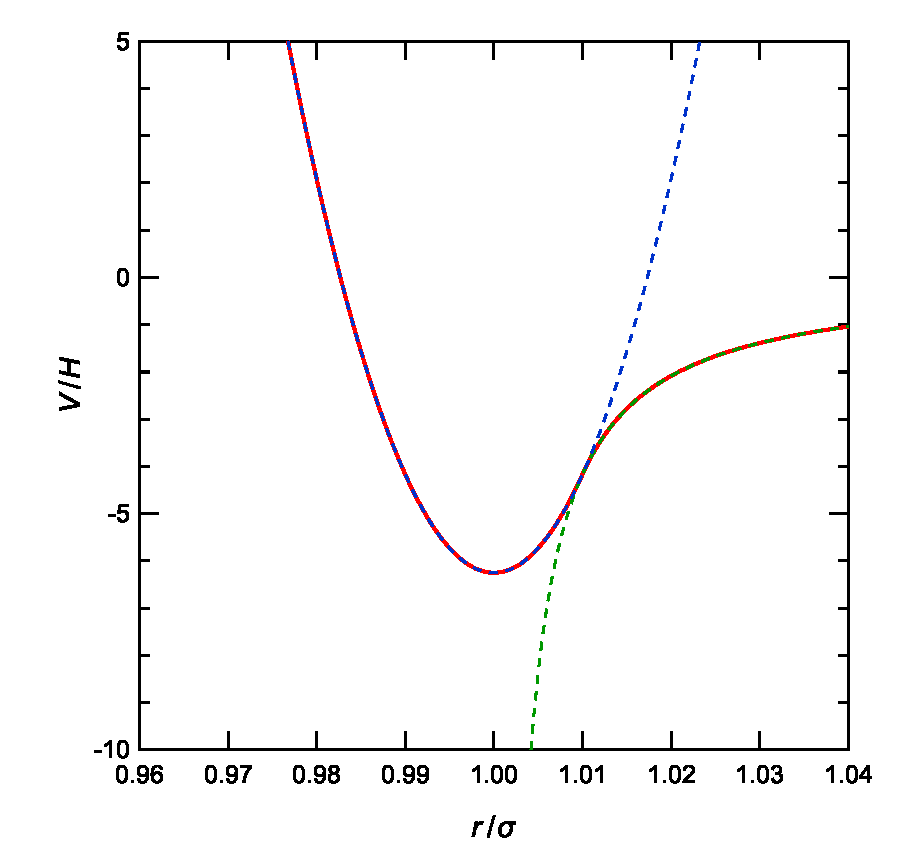
\includegraphics[width=10truecm]{hamaker.pdf}
    \caption{
        斥力を考慮した巨視的粒子間相互作用ポテンシャル(赤の実線).青の破線はソフト斥力ポテンシャルを表し,緑の破線はHamakerによる粒子間相互作用ポテンシャルを表す.}
    \label{fig:hamaker}
\end{figure}

\subsection{シミュレーションにおける単位}
\label{sec:simulation_unit}
拡張KAPSELでの長さと時間の単位は,オリジナルのKAPSELの設定を踏襲し,それぞれ格子幅$\Delta$と粘性拡散時間$\tau = \rho \Delta^2 / \eta$となっている.
また,シミュレーションの時間刻みの自動設定値$\Delta t$もオリジナルのKAPSEL設定と同一である.
つまり,$\Delta t = T_{\mathrm {dump}} = \rho / k_{\mathrm{max}}^2 \eta$である.
ここで,$k_{\mathrm{max}}$は,流体計算の解像度を表す最大波数である.
通常はこの自動設定値を利用すればよいが,計算が不安定な場合は,調整パラメータ$factor$を使って時間刻みを小さくすることができる.
この調整パラメータを設定することで,シミュレーションの時間刻みは,$\Delta t = T_{\mathrm {dump}} \times factor$として与えられるようになる.

\section{シミュレーションの設定}
\subsection{入力用UDFファイルの設定}

入力用UDFファイルは,シミュレーション条件のパラメータが記述されたファイルである.
\ref{sec:kapsel_sample}章のサンプル例では,input.udfが入力用UDFファイルである.
入力用UDFファイルは,OCTAに付属するGOURMETで開くことで編集できる(図\ref{fig:gourmet_input}).

\begin{figure}[htbp]
    \centering
    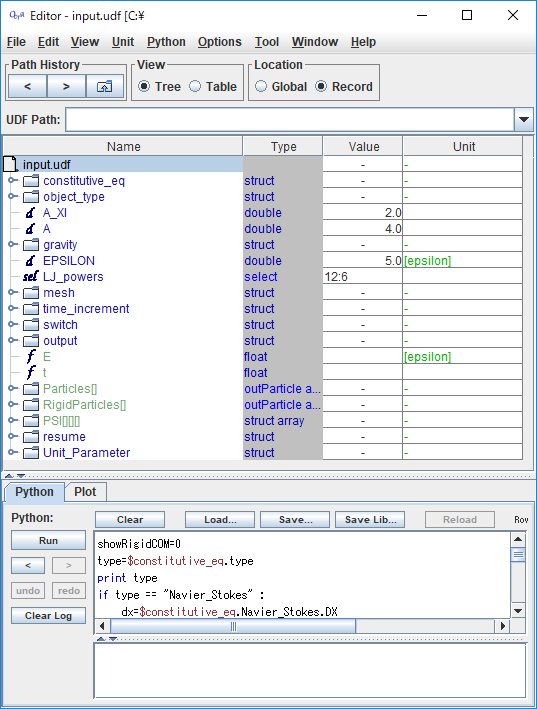
\includegraphics[width=10truecm]{gourmet_input_ss.png}
    \caption{Gourmetによる入力用UDFファイルの編集}
    \label{fig:gourmet_input}
\end{figure}

\verb|constitutive_eq|の設定では,シミュレーションの種類を選ぶことができる.
\verb|type|の項目で設定可能なシミュレーションタイプの一覧を表\ref{tab:constitutive_eq_type}に示す.
表中灰色で示したシミュレーション設定は,オリジナルのKAPSELと同じものであり,MPI並列対応版KAPSELで選択できる.
これらのパラメータの設定については,オリジナルのKAPSELのドキュメント\autocite{shinkagaku2017octa}を参照頂きたい.

\begin{table}[htbp]
    \centering
    \caption{拡張KAPSELで設定可能なシミュレーションの種類}
    \begin{tabular}{ll}
        \toprule
        \verb|constitutive_eq.type| & 説明 \\
        \cmidrule(r){1-1}
        \cmidrule(r){2-2}
        \rowcolor{lightgray!60}
        \verb|Navier_Stokes| & 初期流れ場なし \\
        \rowcolor{lightgray!60}
        \verb|Shear_Navier_Stokes| & ジグザグ流れのせん断流あり \\
        \rowcolor{lightgray!60}
        \verb|Shear_Navier_Stokes_Lees_Edwards| & Lees--Edwards(LE)境界条件のせん断流あり \\
        \rowcolor{lightgray!60}
        \verb|Electrolyte| & 荷電粒子シミュレーション \\
        \verb|Navier_Stokes_FDM| & 初期流れ場なし(差分法) \\
        \verb|Navier_Stokes_Cahn_Hilliard_FDM| & 初期流れ場なし/二成分流体\\
        \verb|Shear_Navier_Stokes_Lees_Edwards_FDM| & LE境界条件のせん断流あり(差分法) \\
        \verb|Shear_NS_LE_CH_FDM| & LE境界条件のせん断流あり/二成分流体 \\
        \bottomrule
    \end{tabular}
    \label{tab:constitutive_eq_type}
\end{table}

\verb|constitutive_eq.type|でシミュレーションの種類を指定すると,各シミュレーションの種類ごとに設定が必要な項目が表示される.
まず,最も基本的なシミュレーションである,\verb|Navier_Stokes_FDM|での設定項目を表\ref{tab:navier_stokes_fdm}に示す.

\begin{table}[htbp]
    \centering
    \cprotect\caption{\verb|Navier_Stokes_FDM|の設定項目}
    \begin{tabular}{lll}
        \toprule
        設定項目 & \multicolumn{2}{l}{説明} \\
        \cmidrule(r){1-1}
        \cmidrule(r){2-3}
        \verb|NS_solver| & \multicolumn{2}{l}{Navier--Stokesソルバーの計算手法の選択} \\
        & \multicolumn{2}{l}{(\UseVerb{verb_exp} / \UseVerb{verb_imp})} \\
        \rule{0pt}{4ex}
        & \UseVerb{verb_imp} の設定項目 & 説明\\
        \cmidrule(r){2-2}
        \cmidrule(r){3-3}
        & \verb|tolerance| & 収束判定基準 \\
        & \verb|maximum_iteration| & 最大反復回数 \\
        \rule{0pt}{6ex}
        \verb|DX| & \multicolumn{2}{l}{格子幅} \\
        \verb|RHO| & \multicolumn{2}{l}{流体の密度} \\
        \verb|ETA| & \multicolumn{2}{l}{流体の粘度} \\
        \verb|kBT| & \multicolumn{2}{l}{粒子温度} \\
        \verb|alpha_v| & \multicolumn{2}{l}{粒子の並進温度に対する補正項} \\
        \verb|alpha_o| & \multicolumn{2}{l}{粒子の回転温度に対する補正項} \\
        \bottomrule
    \end{tabular}
    \label{tab:navier_stokes_fdm}
\end{table}
\verb|NS_solver|の設定では,NS方程式の計算手法の選択ができる.
\verb|explicit_scheme|を選ぶと陽解法が,\verb|implicit_scheme|を選ぶと陰解法が設定される.
それらの計算手法の詳細は\ref{sec:navier_stokes_solver}節に示している.
\verb|implicit_scheme|を選ぶと,デフォルトで線形連立方程式の反復解法としてBiCGSTAB法が選択されるとともに,表中に示す新たな設定項目が現れる.
陰解法の反復解法では,残差のオーダーが\verb|tolerance|で設定した値より小さくなると,解が収束したと判定される.
また,\verb|maximum_iteration|よりも反復回数が多くなると解が得られなかったと判定され,シミュレーションは終了される.

\verb|Navier_Stokes_Cahn_Hilliard_FDM|の設定項目は,表\ref{tab:navier_stokes_fdm}に示す\verb|Navier_Stokes_FDM|に加えて,新たに以下の表\ref{tab:navier_stokes_cahn_hilliard_fdm}に示す二成分流体に関する設定が追加されている.
\verb|NS_solver|の設定では,\verb|implicit_scheme|を選ぶことで粘度比の導入ができる.
\verb|viscosity_change|を\verb|ON|にすると,二成分流体それぞれのバルクの粘度\verb|ETA_A|と\verb|ETA_B|を設定する項目が現れる.
ここで,二成分流体の中間の組成をもつ流体界面領域の粘度は,\verb|ETA_A|と\verb|ETA_B|の線形混合で表される.
\ref{sec:simulation_unit}節に示すように,シミュレーションの時間刻みは\verb|ETA|で設定され,ここで設定する二成分流体の粘度は時間刻みに影響を与えない.
そのため,\verb|ETA|より極端に大きな\verb|ETA_A|と\verb|ETA_B|を設定すると,シミュレーション精度が悪化したり,計算不安定となる可能性があることに注意する.

\verb|CH_solver|の設定では,CH方程式の計算手法の選択ができる.
\verb|explicit_scheme|を選ぶと陽解法が,\verb|implicit_scheme|を選ぶと陰解法が設定される.
それらの計算手法の詳細は\ref{sec:cahn_hilliard_solver}節に示している.
また,\verb|Potential|では,式(\ref{eq:GL_free_energy})に示すGL自由エネルギーのパラメータを設定できる.
\verb|composition_ratio|は二成分流体の組成比を与える.
このパラメータは,後述の二重井戸型ポテンシャルと対応して,適切な範囲で定める必要がある.
\verb|initial_fluctuation|は,初期の濃度ゆらぎの大きさを与える.
設定した平均組成を中心に,\verb|initial_fluctuation|で与えた範囲の一様乱数により,初期濃度場が生成される.
二重井戸型ポテンシャルとしては,Landau型の4次関数によるポテンシャルと,Flory--Huggins型ポテンシャルを選択でき,それぞれ各項のパラメータをここで与えることができる.
これらのポテンシャルの表式は,\ref{sec:phase_separation}節に示している.

\begin{longtable}{lll}
    \caption{二成分流体に関する追加の設定項目}\label{tab:navier_stokes_cahn_hilliard_fdm}\\
    \toprule
    設定項目 & \multicolumn{2}{l}{説明} \\
    \cmidrule(r){1-1}
    \cmidrule(r){2-3}
    \verb|NS_solver| & \multicolumn{2}{l}{Navier--Stokesソルバーの計算手法の選択} \\
    & \multicolumn{2}{l}{(\UseVerb{verb_exp} / \UseVerb{verb_imp})} \\
    \rule{0pt}{4ex}
    & \UseVerb{verb_imp} の設定項目 & 説明\\
    \cmidrule(r){2-2}
    \cmidrule(r){3-3}
    & \verb|tolerance| & 収束判定基準 \\
    & \verb|maximum_iteration| & 最大反復回数 \\
    & \verb|viscosity_change| & 粘度比の導入 (\verb|ON| / \verb|OFF|)\\
    & & \verb|ON|の場合,さらに二成分流体それぞれの粘度\verb|ETA_A|と\\
    & & \verb|ETA_B|を設定する\\
    \rule{0pt}{6ex}
    \verb|CH_solver| & \multicolumn{2}{l}{Cahn--Hilliardソルバーの計算手法の選択} \\
    & \multicolumn{2}{l}{(\UseVerb{verb_exp} / \UseVerb{verb_imp})} \\
    \rule{0pt}{4ex}
    & \UseVerb{verb_imp} の設定項目 & 説明\\
    \cmidrule(r){2-2}
    \cmidrule(r){3-3}
    & \verb|tolerance| & 収束判定基準 \\
    & \verb|maximum_iteration| & 最大反復回数 \\
    \rule{0pt}{6ex}
    \verb|Potential| & \multicolumn{2}{l}{二成分流体相分離ポテンシャルの選択} \\
    & \multicolumn{2}{l}{(\UseVerb{verb_landau} / \UseVerb{verb_flory_huggins})} \\
    \rule{0pt}{4ex}
    & 共通の設定項目 & 説明\\
    \cmidrule(r){2-2}
    \cmidrule(r){3-3}
    & \verb|composition_ratio| & 組成比 \\
    & \verb|initial_fluctuation| & 初期濃度ゆらぎ \\
    & \verb|d| & 粒子領域の流体部分を中立組成に保つためのパラメータ \\
    & \verb|w| & 粒子--流体間相互作用のパラメータ \\
    & \verb|alpha| & 流体--流体界面の相互作用パラメータ \\
    & \verb|kappa| & 易動度 \\
    \rule{0pt}{4ex}
    & \UseVerb{verb_landau} の設定項目 & \\
    \cmidrule(r){2-2}
    & \verb|a| & 4次の項のパラメータ \\
    & \verb|b| & 2次の項のパラメータ \\
    & \UseVerb{verb_flory_huggins} の設定項目 & \\
    \cmidrule(r){2-2}
    & \verb|na| & A成分の重合度 \\
    & \verb|nb| & B成分の重合度 \\
    & \verb|chi| & Floryの相互作用パラメータ \\
    \bottomrule
\end{longtable}

\verb|Shear_Navier_Stokes_Lees_Edwards_FDM|を選択した場合,表\ref{tab:navier_stokes_fdm}に示す\verb|Navier_Stokes_FDM|の設定に加えて,以下の表\ref{tab:shear_parameters}に示すせん断流れに関するオプションが追加される.

\begin{longtable}{lll}
    \caption{せん断流れに関する追加の設定項目}\label{tab:shear_parameters}\\
    \toprule
    設定項目 & \multicolumn{2}{l}{説明} \\
    \cmidrule(r){1-1}
    \cmidrule(r){2-3}
    \verb|External_field| & \multicolumn{2}{l}{せん断流動の種類の選択} \\
    & \multicolumn{2}{l}{(\UseVerb{verb_dc} / \UseVerb{verb_ac})} \\
    \rule{0pt}{4ex}
    & \UseVerb{verb_dc} の設定項目 & 説明\\
    \cmidrule(r){2-2}
    \cmidrule(r){3-3}
    & \verb|Shear_rate| & 定常せん断速度 \\
    \rule{0pt}{4ex}
    & \UseVerb{verb_ac} の設定項目\\
    \cmidrule(r){2-2}
    & \verb|Shear_rate| & 最大振動せん断速度 \\
    & \verb|frequency| & 振動数 \\
    \bottomrule
\end{longtable}

\verb|Shear_NS_LE_CH_FDM|を選択した場合,表\ref{tab:navier_stokes_fdm}に示す\verb|Navier_Stokes_FDM|に加えて,表\ref{tab:navier_stokes_cahn_hilliard_fdm}と\ref{tab:shear_parameters}に示すせん断流れに関するオプションが追加される.
それらの設定は上記した方法と同様である.

\verb|object_type|の設定では,分散粒子の種類に関する設定ができる.
これらの設定は,オリジナルのKAPSELの設定と同じものである.
表\ref{tab:object_parameters}にその概要を示す.

\begin{longtable}{lll}
    \caption{分散粒子の種類に関する項目}\label{tab:object_parameters}\\
    \toprule
    設定項目 & \multicolumn{2}{l}{説明} \\
    \cmidrule(r){1-1}
    \cmidrule(r){2-3}
    \verb|object_type.type| & \multicolumn{2}{l}{固体粒子の種類の選択} \\
    & \multicolumn{2}{l}{(\UseVerb{verb_spherical_particle} / \UseVerb{verb_chain} / \UseVerb{verb_rigid})} \\
    \rule{0pt}{4ex}
    & \UseVerb{verb_spherical_particle} の設定項目 & 説明\\
    \cmidrule(r){2-2}
    \cmidrule(r){3-3}
    & \verb|Particle_number| & 粒子数 \\
    & \verb|MASS_RATIO| & 粒子密度/流体密度 \\
    & \verb|Sarface_charge| & 粒子表面電荷の帯電量 \\
    & & \verb|constitutive_eq.type = Electrolyte|\\
    & & のとき有効\\
    & \verb|janus_*| & 自己推進粒子のパラメータ\\
    & & デフォルトでは,\verb|janus_axis = NONE|\\
    & & \verb|janus_propulsion = OFF|が設定される\\
    \rule{0pt}{4ex}
    & \UseVerb{verb_chain} の設定項目\\
    \cmidrule(r){2-2}
    & \verb|Beads_number| & 1本の鎖に属するビーズ数 \\
    & \verb|Chain_number| & 鎖の本数 \\
    & \verb|MASS_RATIO| & ビーズ密度/流体密度 \\
    & \verb|Sarface_charge| & ビーズ表面電荷の帯電量 \\
    & & \verb|constitutive_eq.type = Electrolyte|\\
    & & のとき有効\\
    & \verb|janus_*| & 自己推進粒子のパラメータ(ここでは省略) \\
    \rule{0pt}{4ex}
    & \UseVerb{verb_rigid} の設定項目\\
    \cmidrule(r){2-2}
    & \verb|Beads_number| & 1つの剛体を構成する球の数 \\
    & \verb|Chain_number| & 剛体の数 \\
    & \verb|MASS_RATIO| & 球密度/流体密度 \\
    & \verb|Rigid_motion| & \verb|free|: 自由運動 \\
    & & \verb|fix|: 指定した速度(\verb|Rigid_velocity|)・\\
    & & \qquad~角速度(\verb|Rigid_omega|)で運動\\
    \bottomrule
\end{longtable}

粒子に関する設定や,シミュレーションや分散粒子の種類によらないグローバルなパラメータは,共通パラメータとして設定する.
これらのパラメータは,オリジナルのKAPSELと同様である.
表\ref{tab:global_parameters}に一覧を示す.
\verb|LJ_powers|の設定では,LJポテンシャルのべき指数の設定だけでなく,Hamakerによる巨視的粒子間ポテンシャルにソフトな斥力を組み合わせたポテンシャル \verb|macro_vdw|が設定できる.
このポテンシャルの詳細は\ref{sec:dlvo}節に示した.
$n$の値については,\verb|interaction.h|の\verb|Lennard_Jones_f|関数内で直接設定する.
また,このポテンシャルを選択すると,\verb|EPSILON|で与えるパラメータがHamaker定数となる.

\begin{longtable}{ll}
    \caption{共通パラメータの一覧}\label{tab:global_parameters}\\
    \toprule
    設定項目 & 説明 \\
    \cmidrule(r){1-1}
    \cmidrule(r){2-2}
    \verb|A_XI| & 粒子界面の厚さ$\xi$\\
    \verb|A| & 粒子半径 \\
    \verb|gravity.G| & 重力加速度 \\
    \verb|gravity.direction| & 重力が印加される方向 (\verb|-X| / \verb|-Y| / \verb|-Z|) \\
    \verb|EPSILON| & 粒子間相互作用であるLennard-Jones(LJ)ポテンシャルのエネルギーの大きさ \\
    \verb|LJ_powers| & LJポテンシャルのべき指数の設定,あるいは巨視的粒子間ポテンシャルの設定\\
    & (\verb|12:6| / \verb|24:12| / \verb|36:18|/ \verb|macro_vdw|) \\
    \verb|mesh.NPX| & シミュレーションセルの$x$方向のサイズ $L_{\mathrm x} = 2^{\UseVerb{verb_npx}}$\\
    \verb|mesh.NPY| & シミュレーションセルの$y$方向のサイズ $L_{\mathrm y} = 2^{\UseVerb{verb_npy}}$\\
    \verb|mesh.NPZ| & シミュレーションセルの$z$方向のサイズ $L_{\mathrm z} = 2^{\UseVerb{verb_npz}}$\\
    \verb|time_increment.type| & 時間刻みの設定 \\
    & \verb|auto|: $\Delta t = T_{\mathrm {dump}} \times \UseVerb{verb_factor}$に設定 \\
    & \verb|manual|: 任意の値に設定 \\
    \bottomrule
\end{longtable}

また,シミュレーションの実行条件の設定一覧を表\ref{tab:simulation_settings}に示す.
二成分流体対応の拡張KAPSELでは,相構造等のフィールドデータは自動的にHDF5フォーマットで出力される.

\begin{longtable}{ll}
    \caption{シミュレーションの実行条件の一覧} \label{tab:simulation_settings}\\
    \toprule
    設定項目 & 説明 \\
    \cmidrule(r){1-1}
    \cmidrule(r){2-2}
    \verb|switch.ROTATION| & 粒子の回転運動の有無 (\verb|ON| / \verb|OFF|)\\
    \verb|switch.LJ_truncate| & LJポテンシャルの引力項の有無 (\verb|ON| / \verb|OFF| / \verb|NONE|)\\
    & \verb|NONE|の場合,相互作用しない幽霊粒子となる \\
    \verb|switch.INIT_distribution| & 粒子の初期配置の設定 \\
    & (\verb|uniform_random| / \verb|random_walk| / \verb|FCC| / \verb|BCC| / \verb|user_specify|)\\
    & \verb|uniform_random|: ランダムに配置 \\
    & \verb|random_walk|: 正方格子から\verb|random_walk.iteration|回ランダムに\\
    & \hspace{14.5ex} 粒子を変位させて配置\\
    & \verb|FCC|: FCC格子上に配置 \\
    & \verb|BCC|: BCC格子上に配置 \\
    & \verb|user_specify|: 座標と速度を以下のリストでユーザー定義する\\
    & \hspace{15.5ex} 座標: \verb|user_specify.Particles[].R| \\
    & \hspace{15.5ex} 速度: \verb|user_specify.Particles[].v| \\
    \verb|switch.INIT_orientation| & 粒子の配向の設定 \\
    &(\verb|user_specify| / \verb|random| / \verb|space_align|) \\
    & \verb|user_specify|: 配向を以下のリストでユーザー定義する\\
    & \hspace{15.5ex} 座標: \verb|user_specify.Particles[].q| \\
    & \hspace{15.5ex} \verb|switch.INIT_distribution|が\verb|user_specify|に設定\\
    & \hspace{15.5ex} されていないとき,以下の\verb|space_align|と同様の設定\\
    & \hspace{15.5ex} となる\\
    & \verb|random|: ランダム配向 \\
    & \verb|space_align|: 1方向に配向 \\
    \verb|SLIP_*| & 自己推進粒子の界面滑りの設定(ここでは省略)\\
    \verb|switch.FIX_CELL.x| & 系の$x$方向のドリフト補正の有無 (\verb|ON| / \verb|OFF|)\\
    \verb|switch.FIX_CELL.y| & 系の$y$方向のドリフト補正の有無 (\verb|ON| / \verb|OFF|)\\
    \verb|switch.FIX_CELL.z| & 系の$z$方向のドリフト補正の有無 (\verb|ON| / \verb|OFF|)\\
    \verb|pin*| & 粒子のピンニングの設定\\
    & デフォルトで\verb|pin.type = NO|が設定される\\
    \verb|free_rigid*| & 剛体の自由度の設定\\
    & デフォルトで\verb|free_rigid.type = NO|が設定される\\
    \verb|ns_solver.OBL_INT| & LE境界条件のせん断流動シミュレーションにおける座標系変換時の近似\\
    & 関数の設定(\verb|linear| / \verb|spline|)\\
    \verb|output.GTS| & データ出力のインターバルのステップ数\\
    \verb|output.Num_snap| & データ出力の回数 (シミュレーションの総ステップ数は$\UseVerb{verb_gts}\times\UseVerb{verb_num_snap}$)\\
    \verb|output.AVS*| & AVS形式のデータ出力の設定 (ここでは省略)\\
    \verb|output.UDF| & 出力UDFデータに時系列データを出力する (\verb|ON| / \verb|OFF|)\\
    \verb|resume.Calculation| & 新規シミュレーションであるか途中から開始されたものであるかのフラグ \\
    & (\verb|NEW| / \verb|CONTINUE_ORIGINAL| / \verb|CONTINUE_FDM| / \\
    & \verb|CONTINUE_FDM_PHASE_SEPARATION|)\\
    & \verb|NEW|: 新規シミュレーション \\
    & \verb|CONTINUE_ORIGINAL|: オリジナルのKAPSELのシミュレーションタイプ\\
    & \hspace{21.5ex} 用のリスタートデータ\\
    & \verb|CONTINUE_FDM|: 拡張KAPSELの差分法相分離なしのシミュレーションタ\\
    & \hspace{15.5ex} イプ用のリスタートデータ\\
    & \verb|CONTINUE_FDM_PHASE_SEPARATION|: 拡張KAPSELの差分法相分離あり\\
    & \hspace{36.0ex} のシミュレーションタイプ用のリ\\
    & \hspace{36.0ex} スタートデータ\\
    \verb|Unit_Parameter.*| & 無次元化の基準となるパラメータの設定\\
    & 無次元化されたシミュレーションパラメータを,GOURMETで実次元\\
    & 表示するためのパラメータ (シミュレーションへの影響は無い)\\
    \bottomrule
\end{longtable}

\subsection{反復解法ライブラリLisを使用するときの設定}
\label{sec:lis_settings}

二成分流体対応の拡張KAPSELでは,反復解法ライブラリLisを利用することで,NS方程式とCH方程式の陰解法において,様々な前処理と反復解法を組み合わせた計算が可能となる.
Makefileで\verb|LIS|オプションを\verb|ON|にすると,自動的に陰解法ソルバーでLisが利用される.
使用する前処理と反復解法の設定は,拡張KAPSELプログラム内に記述する.
\verb|fdm_matrix_solver.cxx|の\verb|Init_lis|関数に,\verb|lis_solver_set_option|の設定箇所が2箇所存在する.
それらはNS方程式とCH方程式の陰解法ソルバーの設定である.
Lisの設定については,該当箇所のコメントに例を示しているが,詳細は公式ユーザーガイド\autocite{lis_document}を参照いただきたい.
%\section*{謝辞}
%この成果は,国立研究開発法人新エネルギー・産業技術総合開発機構(NEDO)の委託業務(P16010)の結果得られたものです.
\printbibliography
\end{document}
